\chapter{Implementation}
\label{chap:implementation}
As outlined in the Chapter 2, ProGENitor is made up of several
different sections.  It contains a database framework to draw data for
analysis.  It has a tool to generate synthetic data for testing.  The core tool
contains algorithms to map out career paths and show important points along the
path.  It also uses Weka to draw some insights about the data that the mapping
algorithms may fail to capture.  ProGENitor would then return the results in an
object such that a user interface could render the information to an end user.
\section{Database}
\label{sect:database}
As ProGENitor needed a method to pull large amounts of data off the backend
server database, a Java method had to be implemented that interfaced with
the database.  MySQL was chosen as it is open source, widely used, and fairly
easy to quickly learn.  Once the MySQL interface was established a wrapper was
added such that another database method could be inserted without a significant
work effort in the rest of the code.  Then, through this wrapper, the many
different function calls were implemented to collect the data needed to generate
the career map and derive any further insights through Weka.

\subsection{MySQL Interface}
To greatly simplify this work, a predefined library jar was added
to the project.  In this case, the library used was SQLite JDBC.  The SQLite
library allows for easy access to a MySQL database for creating, reading from,
writing to, and querying the database.  In the case of ProGENitor, once the
library was added, the code was very straight forward.  Through a couple
commands, the code established the database connection, ran the specified query
or other command, and collected the returned data \cite{sqlite}.  Using the
SQLite library allowed the MySQL interface to quickly add in functions to create
a database, collect query matches from the database, upload lines and files to
the database, modify lines within the database, and even pull the entire
database.  With these functions in place, ProGENitor easily and quickly can
access any defined database.  In the case of ProGENitor, four databases were
generated; one for user profile data, one for education data, one for job data,
and finally one that contains the headers of the other databases.  If, in the
future, additional databases are needed, ProGENitor can easily add them. 
Additionally, as the SQL commands are standard commands, the interface can
easily be replaced with another database interface or expanded upon by anyone
familiar with a SQL language.

\subsection{User Wrapper}
As previously stated, it was desired that ProGENitor be setup such that it was
easy to swap out the database interface with another interface.  Thus, the user
interface wrapper was written to call the various SQL commands.  If in the
future, the database needed to be changed, the work to do so would reside in
adding the database interface and changing the user interface wrapper to point
to the new database.  The wrapper also adds in commands that make interfacing
with the code a bit more clear.  Commands such as add user, database
setup, query matching users, and return headers all allow users working through
other portions of code to understand what the function calls are actually doing
and do not require the developer to necessarily understand the database
interface commands.  Then using these commands, ProGENitor can then collect
data that it passes along to be interpreted by the connections and insights
packages.

\subsection{Data Collection}
With the wrapper and SQL interface in place, ProGENitor then implements a couple
different calls to gather data to be analyzed.  The first of these calls is find
same, in which the code polls the data base for all users that match the query
field value passed to the method.  This method then returns the user IDs in a
TreeSet for all of the users that matched the query.  The next data collection
method available, find all node data, does the same function, but instead
returns all of the matching data in an ArrayList.  The final data collection method available,
database pull, returns in an ArrayList, all of the data associated with the
TreeSet of IDs passed to the method.  These methods are all very similar, but
allow for easy data collection by the mapping and Weka methods within the
connections and insights packages.

\section{Mock Data}
\label{sect:mock-data}
As most end user's databases are not easily accessible and having control over
the data in databases allows for better testing, generating mock data that is
then loaded into a local database was chosen for ProGENitor development. 
ProGENitor is easily attached to any other databases, so this only speeds up the
development process.  To generate this data, a perl script was written that
consumes various data files to obtain possible data values and then randomly
selects the values to populate.  The number of users it generates and many other
variables are also controllable.  Once the script completes it outputs a .csv
containing all of the user data, which can be uploaded to the database through
the database architecture included with ProGENitor.

\subsection{Data Files}
To allow for easily updatable mock data, seperate data files were implemented,
so that the values weren't embedded deep within the data generation code.  There
are two different types of data files.  The first type, simply contains a list
of all possible values.  These values are then simply loaded into an array by
the GenerateData script.  Then, the script will randomly select from this
array when it needs one of these values.  The second type, contains a listing of
possible values dependant on a previous value.  For example, in the line below,
to get a Master's Degree in Circuits or Computer Systems, the user must first
obtain a Bachelor's Degree in Electrical.
\\*
\\*Electrical:Circuits,Computer Systems\\*
\\*
Thus, the code will seach the second file type for the line that meets the
dependancy.  Once the line is found, it will load the possible values into an
array and then randomly select from one of these values.

\subsection{Random Selection}
There are two places the code must randomly select data.  The first is the
data that is loaded for each node.  This random selection simply places the data
from one of the data files into an array and uses the Perl rand function to
randomly select an array index value to pull the data from.  This data is then
applied to the individual user's node and then when the node has all necessary
data generated, it is loaded into the Users.csv file.  This file is then later
uploaded into the database.
\\
The second place that code must randomly select data is when it is determining
if a user enters a node or not on each pass.  There are four possible nodes that
a user could enter each pass and each pass they could potentially enter up to
all of the nodes.  These nodes are an undergraduate degree, a masters degree, a
PHD, and a job.  For each of these nodes, a chance value is assigned in the
variables at the top of the script.  Then essentially a 10 sided dice is rolled
at each node, this is done by loading 1 through 10 into an array and applying
the Perl rand function to the array.  If the dice roll is greater than the
predefined chance value, the node is entered and data is generated.  When any
node is entered, all educational chance values are incremented by 1.  This means
it will be much less likely someone will get an advanced degree as their career
progresses.  Additionally, each educational degree level is currently limited to
one degree and requires the previous level have been completed.  All of these
variables are adjustable in the code, so many differnet scenerios can be
generated.


\subsection{Code Flow}
Once the data files and random data selection is understood, the code flow is
relatively straight forward.  Essentially, the code just steps through section
by section generating data for each user and loading it into a .csv file that
can later be uploaded into the database.  Figure \ref {fig:data generation}
depicts this process below.

\pagebreak
\usetikzlibrary{shapes,arrows,chains}

\begin{figure}[H]
	\centering
% Start the picture
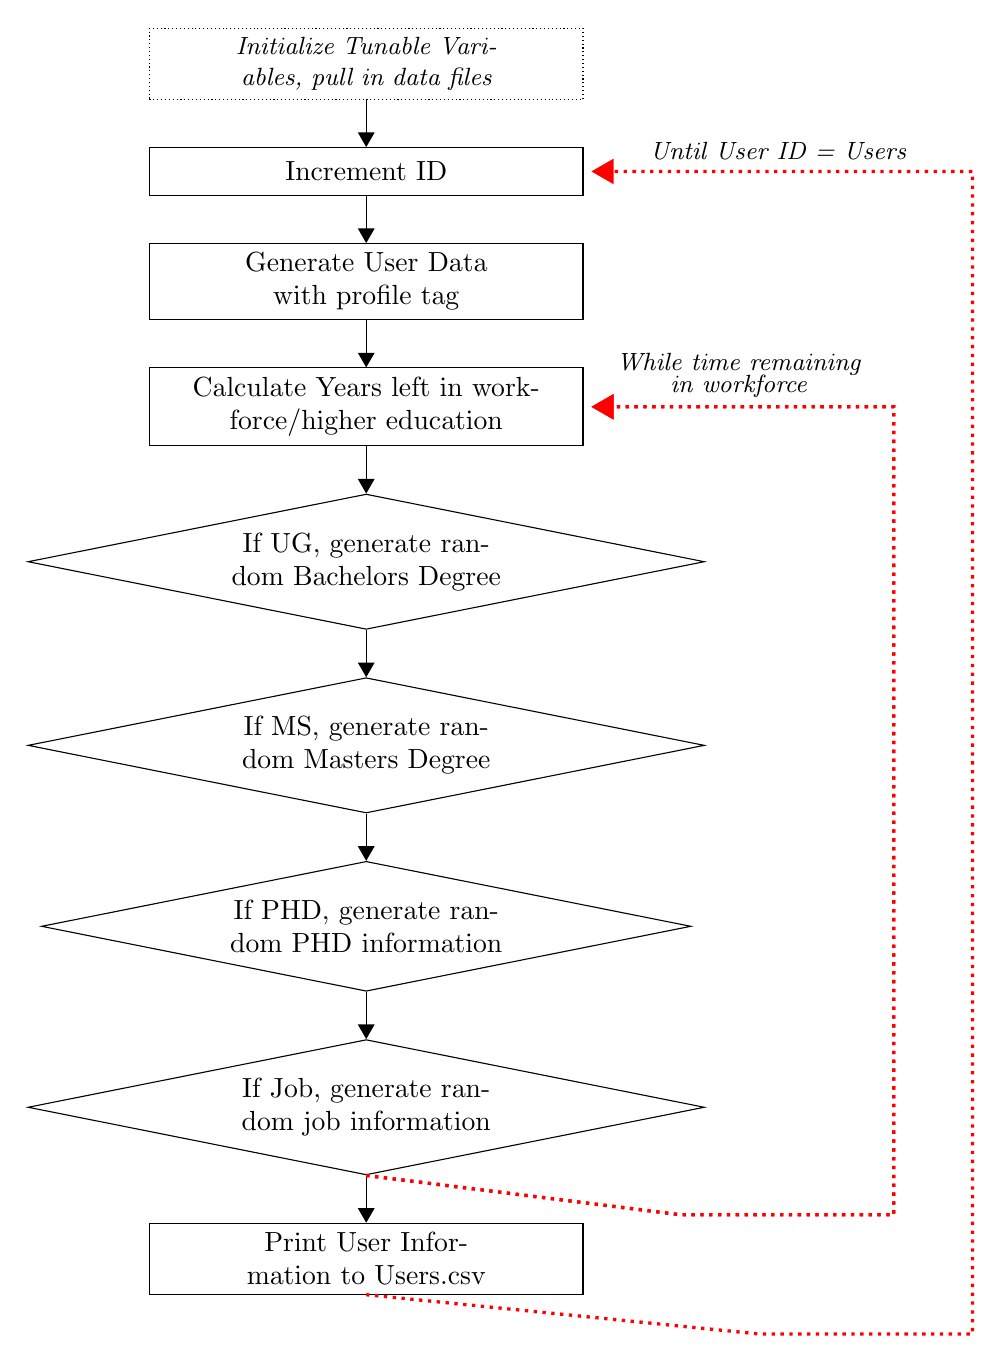
\begin{tikzpicture}[%
    >=triangle 60,              % Nice arrows; your taste may be different
    start chain=going below,    % General flow is top-to-bottom
    node distance=6mm and 60mm, % Global setup of box spacing
    every join/.style={norm},   % Default linetype for connecting boxes
    ]
% ------------------------------------------------- 
% A few box styles 
% <on chain> *and* <on grid> reduce the need for manual relative
% positioning of nodes
\tikzset{
  base/.style={draw, on chain, on grid, align=center, minimum height=4ex},
  proc/.style={base, rectangle, text width=15em},
  test/.style={base, diamond, aspect=5, text width=10em},
  % Connector line styles for different parts of the diagram
  norm/.style={->, draw},
  it/.style={font={\small\itshape}}
}
% -------------------------------------------------
% Start by placing the nodes
\node [proc, densely dotted, it] (p0) {Initialize Tunable Variables, pull in
data files};
% Use join to connect a node to the previous one 
\node [proc, join] (p1) {Increment ID}; 
\node [proc, join] (p2) {Generate User Data with profile tag};
\node [proc, join] (p3) {Calculate Years left in workforce/higher education};
\node [test, join] (t0) {If UG, generate random Bachelors Degree};
\node [test, join] (t1) {If MS, generate random Masters Degree};
\node [test, join] (t2) {If PHD, generate random PHD information};
\node [test, join] (t3) {If Job, generate random job information};
\node [proc, join] (p4) {Print User Information to Users.csv};

\draw [->, dotted, thick, shorten >=1mm] (t3.south) -- ++(40mm,-5mm)  --
++(27mm,0) |- node [black, near end, yshift=0.75em, it]
    [above]{While time remaining}(p3);
    
\draw [->, dotted, thick, shorten >=1mm] (t3.south) -- ++(40mm,-5mm)  --
++(27mm,0) |- node [black, near end, yshift=0.75em, it]
    {in workforce}(p3);

\draw [->, dotted, thick, shorten >=1mm]
  (p4.south) -- ++(50mm,-5mm)  -- ++(27mm,0) 
  |- node [black, near end, yshift=0.75em, it]
    {Until User ID = Users} (p1);

% -------------------------------------------------
\end{tikzpicture}
	\caption{High Level Data Generation}
	\label{fig:data generation}
\end{figure}
\section{Career Paths}
\label{sect:career-paths}
The goal of the career paths module is to generate data, such that a web user
interface could generate a nodal mapping of the career paths taken to reach the
specified career goal.  The node transitions along with the transition
frequencies are returned to the user interface as JSON Objects.  Additionally,
the node ordering and information about each individual node is also returned in
a JSON Object.  This information can then be used to generate a nodal map
depicting various ways of achieving a career goal.  

An example is depicted in figure \ref{fig:nodal map}, which shows various
interconnected nodes that eventually arrive at the goal node, J.  Currently,
each node is labeled with a letter from the alphabet, but ProGENitor would
replace these with actual node names, such as a job title or an educational
degree. The nodes are arranged such that the user most likely travels from left
to right, but the occasional infrequently traveled transition may flow in the
reverse direction.  The frequency that the the path is traveled is depicted
through color in this example.  Red depicts the most frequently traveled path,
then blue, green, and finally the least traveled path is colored black.  Each
node would then be able to display the individual node information upon user
request; either through clicking on the node or through some other user action. 
Note, that ProGENitor does not limit the method in which the user interface is
displayed; it simply passes back statistical information about the nodes, the
transitions between each node, and the individual data about each node.  It is
up to the web user interface developer to determine how the end product is rendered.


\usetikzlibrary{shapes,arrows,chains}

\begin{figure}[H]
	\centering
  
% Start the picture
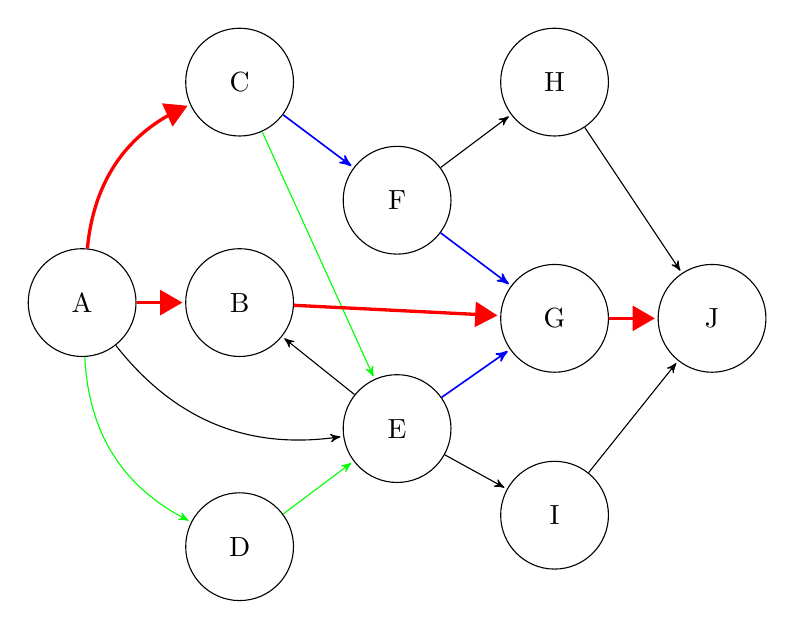
\begin{tikzpicture}[%
    >=triangle 60,              % Nice arrows; your taste may be different
    start chain=going below,    % General flow is top-to-bottom
    node distance=3mm and 20mm, % Global setup of box spacing
    every join/.style={norm},   % Default linetype for connecting boxes
    ]
% ------------------------------------------------- 
% A few box styles 
% <on chain> *and* <on grid> reduce the need for manual relative
% positioning of nodes
\tikzset{
  base/.style={draw, on chain, on grid, align=center, minimum height=2ex},
  node/.style={base, circle, text width=3em},
  % Connector line styles for different parts of the diagram
  norm/.style={->, draw},
  thin/.style={->,>=stealth',shorten >=1pt, black},
  nm/.style={->,>=stealth',shorten >=1pt, green},
  to/.style={->,>=stealth',shorten >=1pt,semithick,blue},
  thick/.style={->,shorten >=1pt,very thick, red},
  it/.style={font={\small\itshape}}
}
% -------------------------------------------------
% Start by placing the nodes
\node [node] (a) {A};
% Use join to connect a node to the previous one 
\node [node, right = of a] (b) {B};
\node [node, above = of b, yshift=25mm] (c) {C}; 
\node [node, below of = b, yshift=-25mm](d) {D};
\node [node, right=of d, yshift =15mm](e) {E};
\node [node, right=of c, yshift=-15mm](f) {F};
\node [node, right=of f, yshift=-15mm](g) {G};
\node [node, right=of f, yshift=15mm](h) {H};
\node [node, right=of f, yshift=-40mm](i) {I};
\node [node, right=of g](j) {J};

\draw[thick] (a) to (b);
\draw[thick] (a) to[bend left=30] (c);
\draw[nm] (a) to[bend right=30] (d);
\draw[nm] (d) to (e); 
\draw[thin] (a) to[bend right=30] (e);
\draw[nm] (c) to (e);
\draw[to] (c) to (f);
\draw[thin] (e) to (b);
\draw[to] (e) to (g);
\draw[to] (f) to (g);
\draw[thick] (b) to (g);
\draw[thin] (f) to (h);
\draw[thin] (e) to (i);
\draw[thick] (g) to (j);
\draw[thin] (h) to (j);
\draw[thin] (i) to (j);

% -------------------------------------------------
\end{tikzpicture}

	\caption{Career Path Nodal Map}
	\label{fig:nodal map}
\end{figure}

\subsection{Node Interconnects}
The node interconnect portion of code finds all of the nodes that
users pass through and the order at which they pass through them.  It then
tallies the number of times all of the users pass along each transition
path to allow for the career map to depict not only the point to point
connections, but also how frequently that path is traveled.  The high level
process to generate this node interconnection data is depicted in figure
\ref{fig:node interconnect} below.


\usetikzlibrary{shapes,arrows,chains}

\begin{figure}[H]
	\centering
% Start the picture
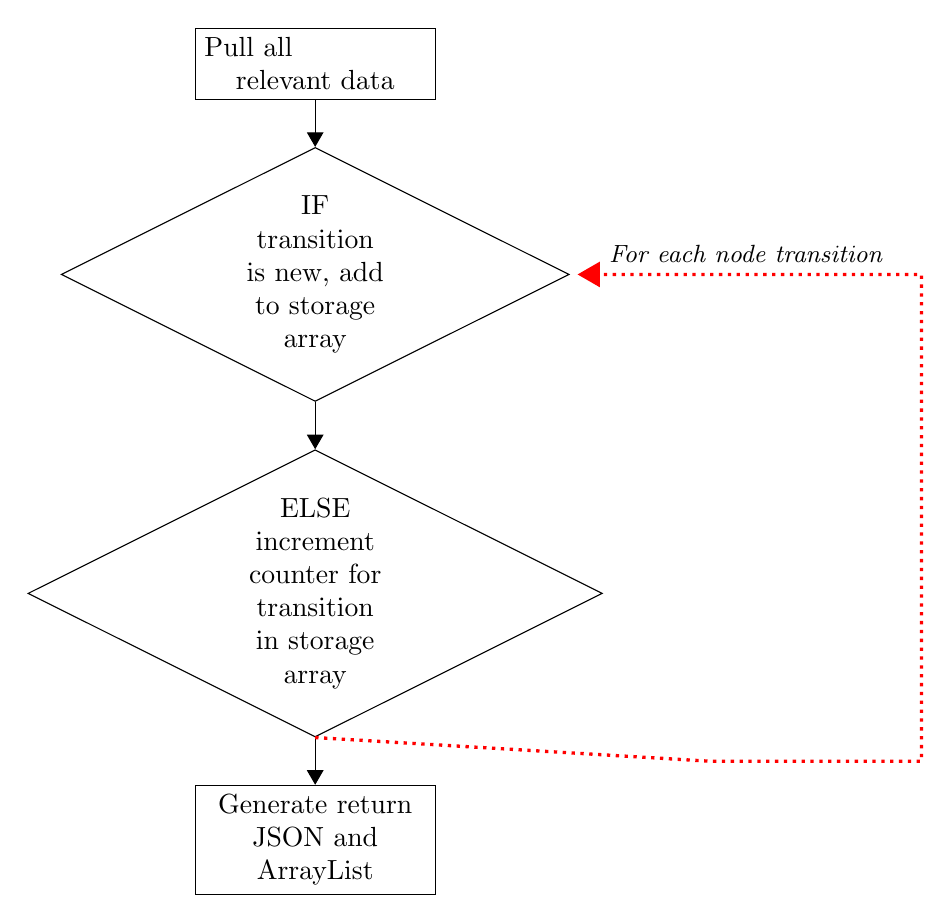
\begin{tikzpicture}[%
    >=triangle 60,              % Nice arrows; your taste may be different
    start chain=going below,    % General flow is top-to-bottom
    node distance=6mm and 60mm, % Global setup of box spacing
    every join/.style={norm},   % Default linetype for connecting boxes
    ]
% ------------------------------------------------- 
% A few box styles 
% <on chain> *and* <on grid> reduce the need for manual relative
% positioning of nodes
\tikzset{
  base/.style={draw, on chain, on grid, align=center, minimum height=4ex},
  proc/.style={base, rectangle, text width=8em},
  test/.style={base, diamond, aspect=2, text width=5em},
  % Connector line styles for different parts of the diagram
  norm/.style={->, draw},
  it/.style={font={\small\itshape}}
}
% -------------------------------------------------
% Start by placing the nodes
\node [proc] (p0) {Pull all\newline relevant data};
% Use join to connect a node to the previous one 
\node [test, join] (t1) {IF transition is new, add to storage array};
\node [test, join] (t2) {ELSE increment counter for transition in storage
array}; 
\node [proc, join](p1) {Generate return JSON and ArrayList};

\draw [->, dotted, thick, shorten >=1mm]
  (t2.south) -- ++(50mm,-3mm)  -- ++(27mm,0) 
  |- node [black, near end, yshift=0.75em, it]
    {For each node transition} (t1);

% -------------------------------------------------
\end{tikzpicture}
	\caption{High Level Node Interconnect Generation}
	\label{fig:node interconnect}
\end{figure}

The process in defining and counting these interconnects was coded in Java in
the find edges method of the connections package.  The process flow is listed
in detail below:

\begin{description}
    \item[Node Interconnect Generation:]
\end{description}
\begin{enumerate}
  \item For each ID passed to Interconnect Generation Module:
  \begin{enumerate}
    \item Pull Job Data and add it to the Nodes Array List.
    \item Pull Education Data and add it to the Nodes Array List.
    \item Set Min equal to MAX Integer and Max equal to MIN Integer.
    \item For each element of the Nodes ArrayList:
    \begin{enumerate}
      \item If date of data for element of Nodes is less than Min and more than
      Max, store the data and set Min equal to date of data.
      \item After all elements of Nodes ArrayList considered, Add stored data
      to User ArrayList and set Max equal to Min.
  	\end{enumerate}
  	\item For each element of User ArrayList:
  	\begin{enumerate}
  	  \item If A is NULL, set A equal to User element node name.
  	  \item Else set B equal to A and set A equal to User element node name.
  	  \item If Connects ArrayList is empty, add B,A,1 to Connects ArrayList.
  	  \item Else check if B,A exists in the Connects ArrayList:
  	  \begin{enumerate}
  	    \item If it exists, increment the counter of the row.
  	    \item If it does not exist, add B,A,1 to the Connects ArrayList.
  	  \end{enumerate}
  	\end{enumerate}
  \end{enumerate}
  \item Push Connects ArrayList containing all node transitions and transition
  counts to a JSON Object containing a JSON Array.
  \item Return both the ArrayList and the JSON Object.
\end{enumerate}

\subsection{Node Ordering}
The node ordering portion of code sorts the nodes such that the major
transitions flow in order from start to finish. It does this so that the flow
of transitions can be mapped in a manner that is not overly confusing.  Figure
\ref{fig:node ordering} shows the high level process that the code follows
to generate the node groupings.  These groupings can then be fed to the end user
interface to order the nodes in a fashion that shows the typical flow of careers
that reach the destination goal.

\usetikzlibrary{shapes,arrows,chains}

\begin{figure}[H]
	\centering
% Start the picture
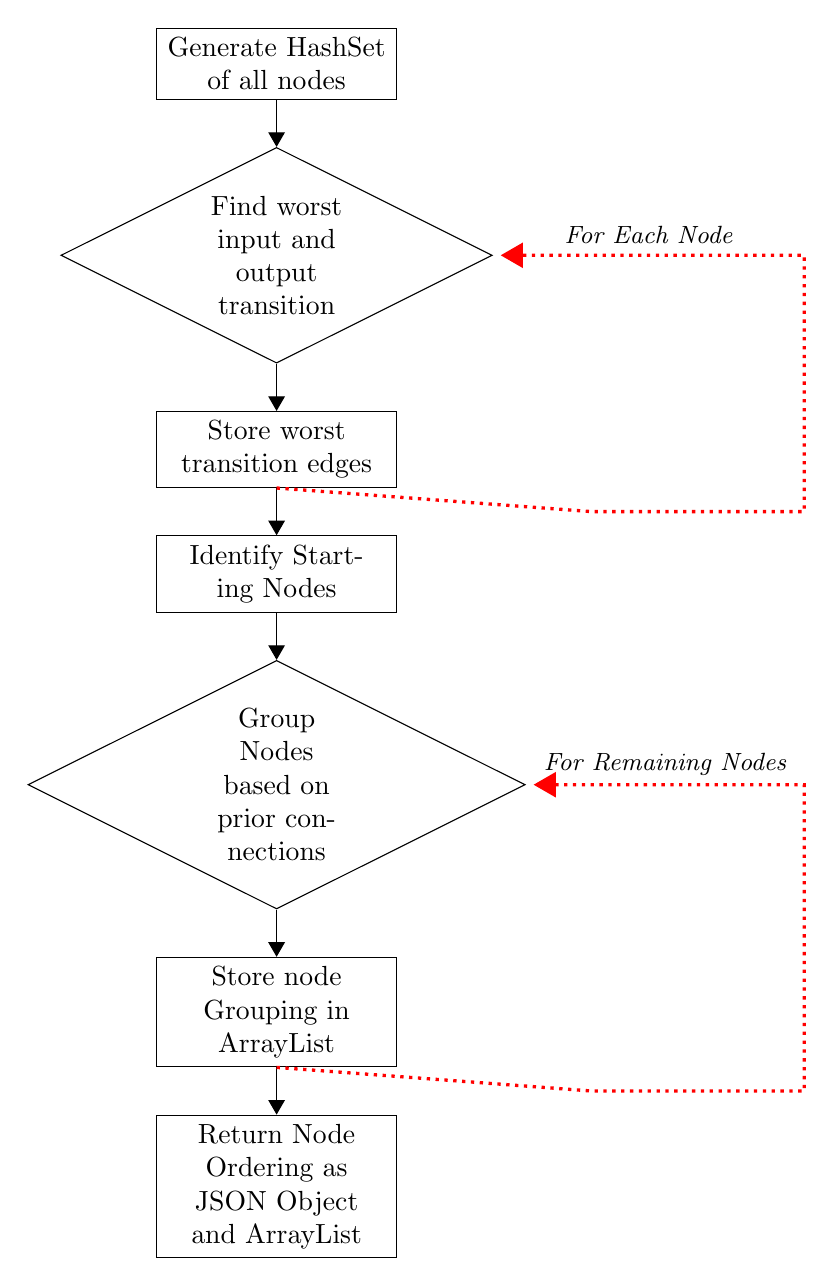
\begin{tikzpicture}[%
    >=triangle 60,              % Nice arrows; your taste may be different
    start chain=going below,    % General flow is top-to-bottom
    node distance=6mm and 60mm, % Global setup of box spacing
    every join/.style={norm},   % Default linetype for connecting boxes
    ]
% ------------------------------------------------- 
% A few box styles 
% <on chain> *and* <on grid> reduce the need for manual relative
% positioning of nodes
\tikzset{
  base/.style={draw, on chain, on grid, align=center, minimum height=4ex},
  proc/.style={base, rectangle, text width=8em},
  test/.style={base, diamond, aspect=2, text width=5em},
  % Connector line styles for different parts of the diagram
  norm/.style={->, draw},
  it/.style={font={\small\itshape}}
}
% -------------------------------------------------
% Start by placing the nodes
\node [proc] (p0) {Generate HashSet of all nodes};
% Use join to connect a node to the previous one 
\node [test, join] (p1) {Find worst input and output transition};
\node [proc, join] (p2) {Store worst transition edges};
\node [proc, join] (p3) {Identify Starting Nodes}; 
\node [test, join] (p4) {Group Nodes based on prior connections};
\node [proc, join] (p5) {Store node Grouping in ArrayList};
\node [proc, join] (p6) {Return Node Ordering as JSON Object and ArrayList};

\draw [->, dotted, thick, shorten >=1mm]
  (p2.south) -- ++(40mm,-3mm)  -- ++(27mm,0) 
  |- node [black, near end, yshift=0.75em, it]
    {For Each Node} (p1);
\draw [->, dotted, thick, shorten >=1mm]
  (p5.south) -- ++(40mm,-3mm)  -- ++(27mm,0) 
  |- node [black, near end, yshift=0.75em, it]
    {For Remaining Nodes} (p4);

% -------------------------------------------------
\end{tikzpicture}
	\caption{High Level Node Order Generation}
	\label{fig:node ordering}
\end{figure}

The process in defining the node ordering for the nodes was coded in Java in the
find node order method of the connections package.  The process flow is listed
in detail below:

\begin{description}
    \item[Node Ordering Generation:]
\end{description}
 \begin{enumerate}
   \item Generate HashSet of All Nodes
   \item For each Node in HashSet:
   \begin{enumerate}
     \item Initialize transitional weight to 0.
     \item For each element of the Node Interconnect Array List:
     \begin{enumerate}
       \item Check if Node matches the input node.
       \item Check if the number of transitions to the node is greater than the
       transitional weight.
       \item If both checks are true; set the transitional weight to the current
       Array List line's number of transitions.
       \item Also, if both checks are true; store this Array List line.
     \end{enumerate}
     \item After the worst input transition is found for the node, store it in
     the Heavy Edges HashSet.
     \item Repeat this entire step for the output nodes.
   \end{enumerate}
   \item For each Heavy Edge element, search the Node Interconnect Array List
   for input nodes that are also destination nodes.
   \begin{enumerate}
     \item Any nodes not found are set as start nodes.
     \item Repeat this step for output nodes that are also starting nodes.  Any
     nodes not found are set as ending nodes.
   \end{enumerate}
   \item Add all the starting nodes to node 0 and add them to the Node Store
   HashSet.
   \item Add all nodes that are not starting nodes to the Remaining Nodes
   HashSet.
   \item Increment the group number to 1.
   \item Until the Remaining Nodes HashSet is empty, loop through the following
   steps.
   \begin{enumerate}
     \item For each Node in Node Store, store all destination nodes in a HashSet
     that Node in Node Store transitions to.
     \item For each destination node stored in the previous step, find all
     possible next destination nodes and check if they are contained within the
     HashSet generated in the previous step.
     \begin{enumerate}
       \item If one is contained within the previously generated HashSet, remove
       the node from the HashSet.
     \end{enumerate}
     \item Add remaining nodes to next node grouping.  Also remove remaining
     nodes from Remaining Nodes HashSet.
     \item Add the node group to the NodeReturn ArrayList.
     \item Increment the group number.
     \item Replace the nodes in the Starting Nodes hash set with the nodes that
     were just added to a group.
   \end{enumerate} 
   \item Generate a JSON Object containing a JSON Array the node groupings from
   the NodeReturn ArrayList.
   \item Return both the JSON Object and the NodeReturn ArrayList.
 \end{enumerate}



\subsection{Node Details}
Presenting all of the potential information would overwhelm any user interface,
so instead many of the details are buried within each node and can be queried
by the end user, by selecting the node of interest.  As each node contains
additional details such as the place of employment or education, time spent at
the school or job, or any other node relevant pieces of information; the data
must be gathered upon user request, as to not slow down the overall map
generation.  Once the request is made, the data about the individuals who
reached the goal node and the data about all of the users who passed through a
particular node are pulled.  This data is then broken down into a statistic for
both cases and compared against each other to determine if something occurred
more frequently for the users who reached the goal node versus those who had
not.  This way any significant differences could be raised to the end user's
attention as potentially important steps to reaching the final goal.  The high
level process to generating this data is depicted in figure \ref{fig:node
details} below.

\usetikzlibrary{shapes,arrows,chains}

\begin{figure}[H]
	\centering
% Start the picture
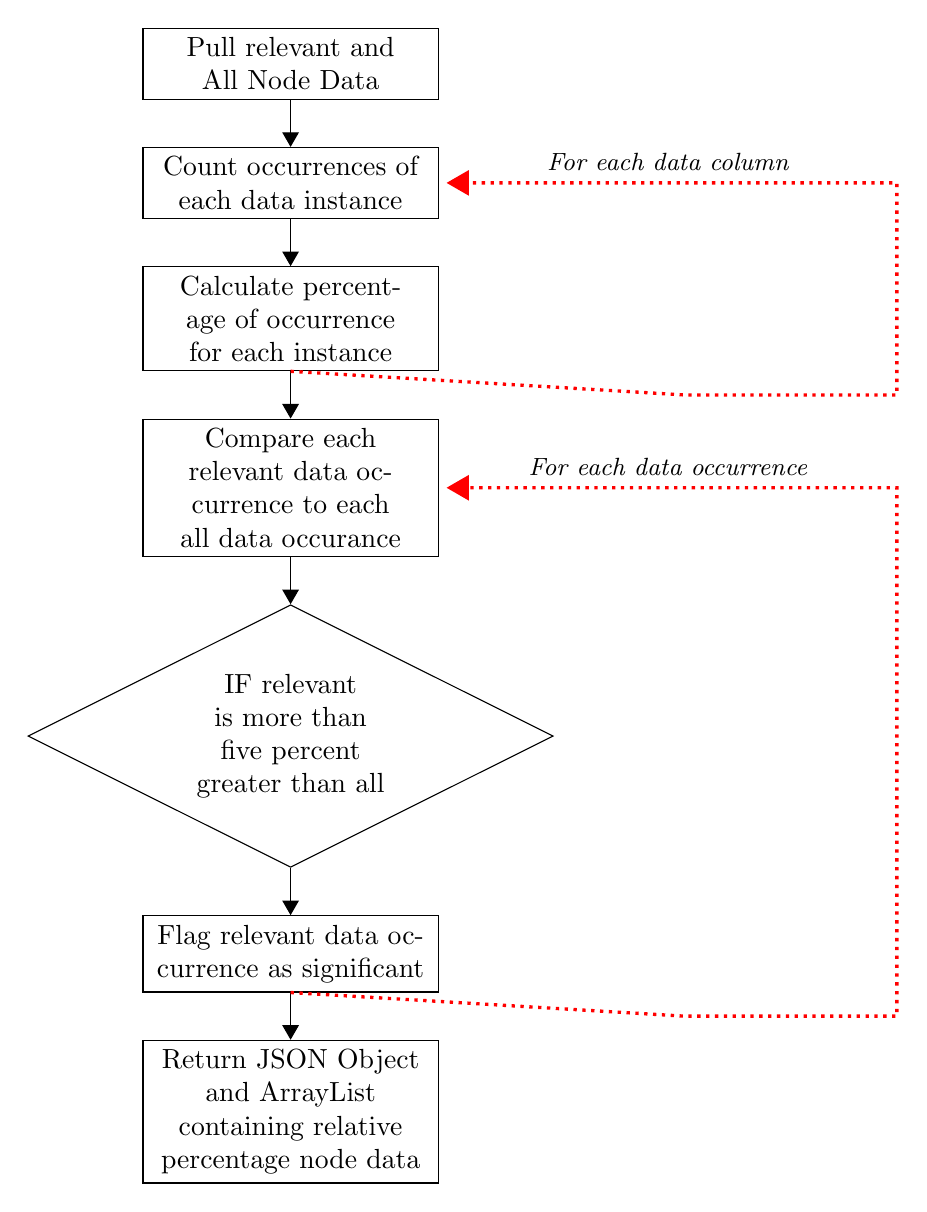
\begin{tikzpicture}[%
    >=triangle 60,              % Nice arrows; your taste may be different
    start chain=going below,    % General flow is top-to-bottom
    node distance=6mm and 60mm, % Global setup of box spacing
    every join/.style={norm},   % Default linetype for connecting boxes
    ]
% ------------------------------------------------- 
% A few box styles 
% <on chain> *and* <on grid> reduce the need for manual relative
% positioning of nodes
\tikzset{
  base/.style={draw, on chain, on grid, align=center, minimum height=4ex},
  proc/.style={base, rectangle, text width=10em},
  test/.style={base, diamond, aspect=2, text width=8em},
  % Connector line styles for different parts of the diagram
  norm/.style={->, draw},
  it/.style={font={\small\itshape}}
}
% -------------------------------------------------
% Start by placing the nodes
\node [proc] (p0) {Pull relevant and All Node Data};
% Use join to connect a node to the previous one 
\node [proc, join] (p1) {Count occurrences of each data instance};
\node [proc, join] (p2) {Calculate percentage of occurrence for each
instance};
 \node [proc, join] (p3) {Compare each relevant data occurrence to each all data
 occurance};
 \node [test, join] (t0) {IF relevant is more than five percent greater than
 all};
 \node [proc, join] (p4) {Flag relevant data occurrence as significant};
 \node [proc, join] (p5) {Return JSON Object and ArrayList containing
 relative percentage node data};

\draw [->, dotted, thick, shorten >=1mm]
  (p2.south) -- ++(50mm,-3mm)  -- ++(27mm,0) 
  |- node [black, near end, yshift=0.75em, it]
    {For each data column} (p1);
\draw [->, dotted, thick, shorten >=1mm]
  (p4.south) -- ++(50mm,-3mm)  -- ++(27mm,0) 
  |- node [black, near end, yshift=0.75em, it]
    {For each data occurrence} (p3);

% -------------------------------------------------
\end{tikzpicture}
	\caption{High Level Node Detail Generation}
	\label{fig:node details}
\end{figure}
\pagebreak

The process in defining the details and significant details for each node was
coded in Java in the find node info method of the connections package.  The
process flow is listed in detail below:

\begin{description}
    \item[Node Detail Generation:]
\end{description}
\begin{enumerate}
  \item Pull in Profile ArrayList, tag each element as a profile, and then add
  the element to the Complete ArrayList.
  \item Repeat this for the Jobs ArrayList and the Education ArrayList.
  \item Check each element of the Complete ArrayList.
  \begin{enumerate}
    \item If the element contains the node that details are being pulled on, add
    the element to the Relevant ArrayList.
  \end{enumerate}
  \item Pull the headers associated with the node that details are being pulled
  from.
  \item Pull all the data in the database for that node and store in the All
  Node Data ArrayList.
  \item For each element of the Complete ArrayList:
  \begin{enumerate}
    \item Split the element into columns and step through each column.
    \begin{enumerate}
    	\item Check if the column element is a start or end year and instead
    	calculate the years spent at the node.
    	\begin{enumerate}
    	  \item If the end year is set to current, find the current year and then
    	  calculate the total years spent at the node.
    	\end{enumerate}
    	\item Add the column value to a HashSet to obtain all possible values for
    	the column.
    	\item Step through the column counting each value instance to obtain a
    	count for each different value.
    	\item Calculate the percentage for each value in the column by diving the
    	count by the total number of elements.
    	\item Push these values into the Relevant ArrayList.
    \end{enumerate} 
  \end{enumerate}
  \item Repeat for each element of the All Node Data Array List
  \item Compare the percentages for each element of the Relevant ArrayList to
  the percentages from the All Node Data Array List.
  \begin{enumerate}
    \item Flag the column value for any instance where the Relevant value's
    percentage exceeds the percentage for all the data by 5\%.
    \item Return this value as relevant so that it can be identified to the user
    as significant to the node.
  \end{enumerate}
  \item Return the Relevant ArrayList and a JSON Object containing a JSON Array
  of the same data.
\end{enumerate}


\section{Weka}
\label{sect:weka}
One of the most popular ways of drawing insights from data through machine
learning is by using a predefined library.  This is because the library takes
much of the technical effort out of the development.  All of the math behind the
machine learning is hidden behind the library and often there are nice user
interfaces or APIs associated with the library.  Typically, there are many
different methods that can be called to comb through the data to extract
insights and relationships about the data.  In the case of ProGENitor the Weka
library was chosen as it has an excellent Java API and access to many different
methods.  Choosing the method to extract information from the data requires some
knowledge about the data itself.  In this case, clustering was chosen as the
data is mostly nominal data and the goal is to define some grouping that leads
to the end goal.  To extract the data, first ProGENitor must generate an
arff file to feed into Weka and then Weka has to evaluate it with the clustering
classification.

\subsection{Arff Creation}
Weka uses the .arff file format to feed data into the Weka tool set.  The arff
file contains two major sections.  These sections are the header section and the
data section \cite{arff}.  The header contains the name of the relation, a list
of attributes, and their types.  The data section contains the data that will
be used for machine learning.  A sample .arff file would look like the
following:\\*
\\*
\begin{tt}
\begin{footnotesize}
@relation education\\*
\\
@attribute degree \{PhD,Bachelors,Masters\}\\*
@attribute specialization
\{Electrical,Circuits,Analog,Computer\newline \indent Architecture,Digital\}\\*
@attribute goal \{true,false\}\\ \\* @data\\*
Bachelors,Electrical,false\\*
Masters,Circuits,false\\*
Bachelors,Electrical,true\\*
Masters,Circuits,true\\*
PhD,MSU,Digital,true\\*
\end{footnotesize}
\end{tt}

ProGENitor currently generates the .arff file containing just the educational
nodes.  One of the keys to getting quality insights out of Weka is controlling
the data being fed into the tools.  In this case, only the educational
data is fed into the tool.  This process could easily be replicated for additional
insights.  To generate the arff file, ProGENitor contains a Java method called
generate arff in the connections package.  This code follows the procedure
detailed in figure \ref{fig:arff generation} to generate the arff file that is
later used by Weka.

\usetikzlibrary{shapes,arrows,chains}

\begin{figure}[H]
	\centering
% Start the picture
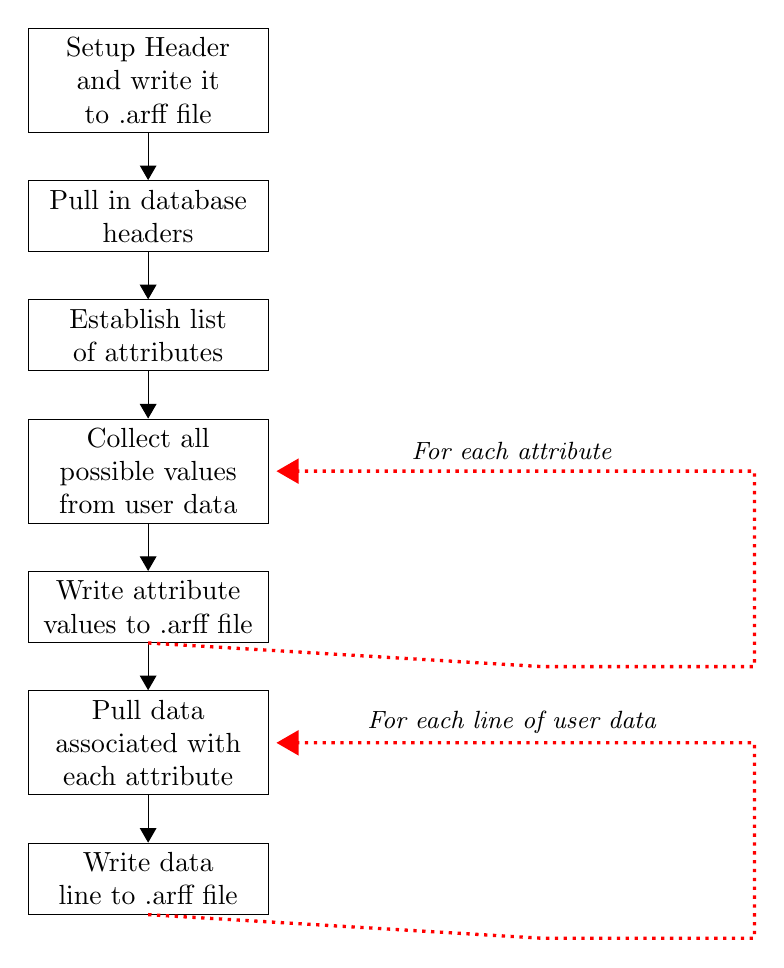
\begin{tikzpicture}[%
    >=triangle 60,              % Nice arrows; your taste may be different
    start chain=going below,    % General flow is top-to-bottom
    node distance=6mm and 60mm, % Global setup of box spacing
    every join/.style={norm},   % Default linetype for connecting boxes
    ]
% ------------------------------------------------- 
% A few box styles 
% <on chain> *and* <on grid> reduce the need for manual relative
% positioning of nodes
\tikzset{
  base/.style={draw, on chain, on grid, align=center, minimum height=4ex},
  proc/.style={base, rectangle, text width=8em},
  test/.style={base, diamond, aspect=2, text width=5em},
  % Connector line styles for different parts of the diagram
  norm/.style={->, draw},
  it/.style={font={\small\itshape}}
}
% -------------------------------------------------
% Start by placing the nodes
\node [proc] (p0) {Setup Header and write it to .arff file};
% Use join to connect a node to the previous one 
\node [proc, join] (p1) {Pull in database headers};
\node [proc, join] (p2) {Establish list of attributes};
\node [proc, join] (p3) {Collect all possible values from user data};
\node [proc, join] (p4) {Write attribute values to .arff file}; 
\node [proc, join] (p5) {Pull data associated with each attribute};
\node [proc, join] (p6) {Write data line to .arff file};

\draw [->, dotted, thick, shorten >=1mm]
  (p4.south) -- ++(50mm,-3mm)  -- ++(27mm,0) 
  |- node [black, near end, yshift=0.75em, it]
    {For each attribute} (p3);

\draw [->, dotted, thick, shorten >=1mm]
  (p6.south) -- ++(50mm,-3mm)  -- ++(27mm,0) 
  |- node [black, near end, yshift=0.75em, it]
    {For each line of user data} (p5);

% -------------------------------------------------
\end{tikzpicture}
	\caption{Arff File Generation}
	\label{fig:arff generation}
\end{figure}

\subsection{Clustering}
One major advantage to using the Weka library is it takes complex code and makes
it relatively simple.  As seen in Figure \ref{fig:clustering}, the process that is
followed to analyze the data in the arff file is very simple and straight
forward.  Once the Weka jar is imported into the project, the code is very quick
to implement, as good documentation is available for the API \cite{weka}.  The
complex portion of work is then ensuring that the appropriate classification is
applied and the data is parsed in a useful fashion.


\usetikzlibrary{shapes,arrows,chains}

\begin{figure}[H]
	\centering
% Start the picture
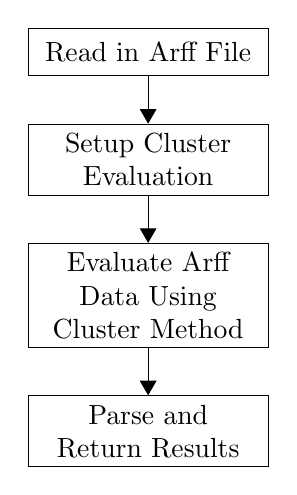
\begin{tikzpicture}[%
    >=triangle 60,              % Nice arrows; your taste may be different
    start chain=going below,    % General flow is top-to-bottom
    node distance=6mm and 60mm, % Global setup of box spacing
    every join/.style={norm},   % Default linetype for connecting boxes
    ]
% ------------------------------------------------- 
% A few box styles 
% <on chain> *and* <on grid> reduce the need for manual relative
% positioning of nodes
\tikzset{
  base/.style={draw, on chain, on grid, align=center, minimum height=4ex},
  proc/.style={base, rectangle, text width=8em},
  test/.style={base, diamond, aspect=2, text width=5em},
  % Connector line styles for different parts of the diagram
  norm/.style={->, draw},
  it/.style={font={\small\itshape}}
}
% -------------------------------------------------
% Start by placing the nodes
\node [proc] (p0) {Read in Arff File};
% Use join to connect a node to the previous one 
\node [proc, join] (p1) {Setup Cluster Evaluation};
\node [proc, join] (p2) {Evaluate Arff Data Using Cluster Method};
\node [proc, join] (p3) {Parse and Return Results};
% -------------------------------------------------
\end{tikzpicture}
	\caption{High Level Data Clustering}
	\label{fig:clustering}
\end{figure}

In the case of ProGENitor, EM (expectation maximization) clustering was chosen
as it automatically determines the number of clusters required through cross
validation.  The algorithm that EM follows is shown in figure
\ref{fig:EM} \cite{EM}.  EM differs from other clustering algorithms in that it
uses probability of cluster membership instead of a distance method used by
other clustering methods such as k-mean clustering.  EM starts with one cluster,
then cross validates the data and applies the probability of cluster membership
classification.  It then calculates the log-likelihood for the set and if it
increases, creates a new cluster and starts over.  It repeats this process until
the log likelihood no longer increases.  The left over clusters will then be
returned as the results.

\begin{figure}[H]
	\centering
% Start the picture
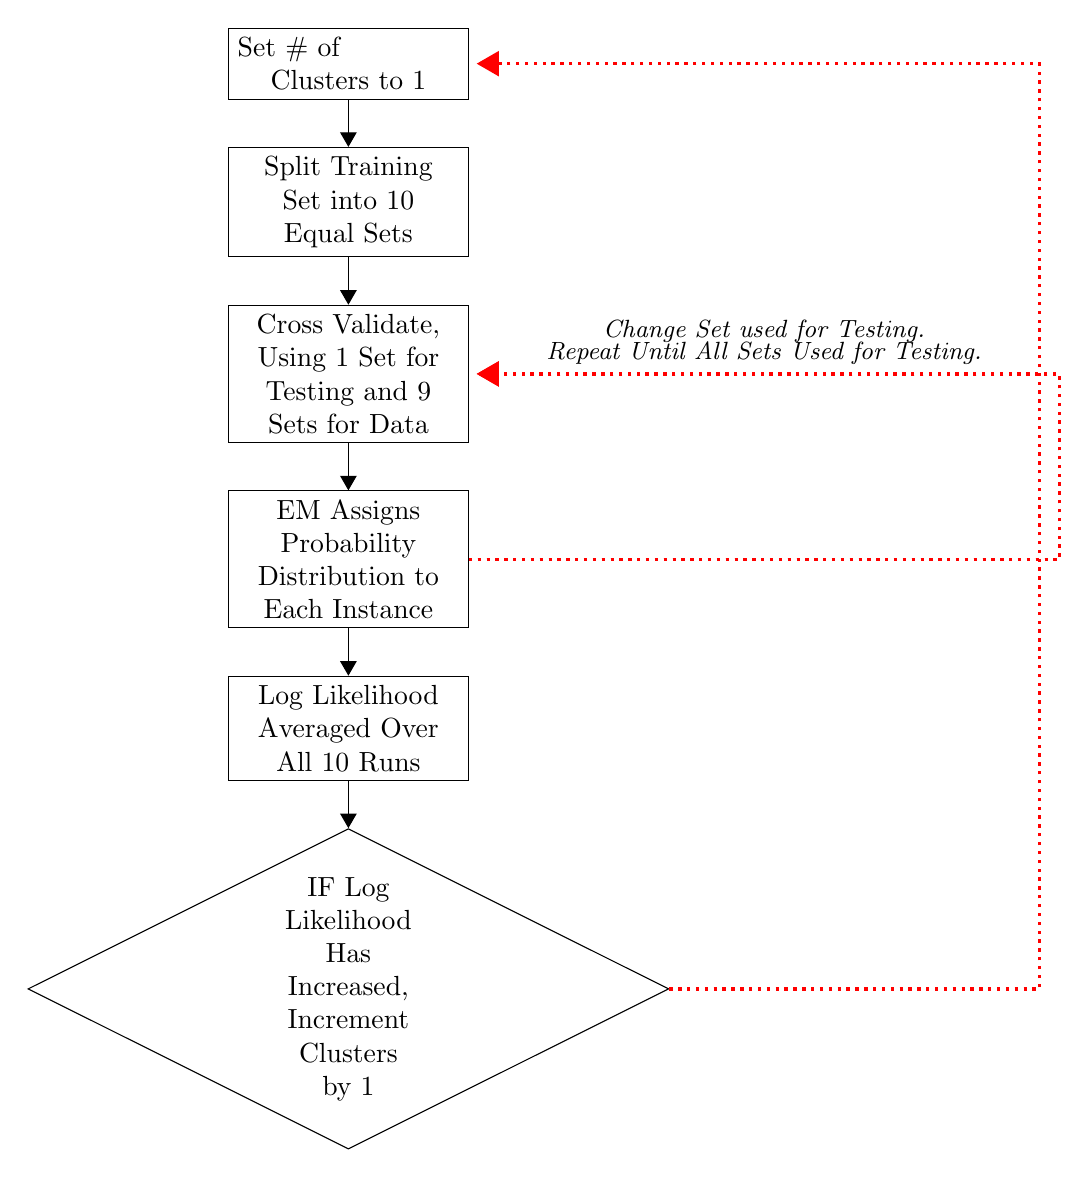
\begin{tikzpicture}[%
    >=triangle 60,              % Nice arrows; your taste may be different
    start chain=going below,    % General flow is top-to-bottom
    node distance=6mm and 60mm, % Global setup of box spacing
    every join/.style={norm},   % Default linetype for connecting boxes
    ]
% ------------------------------------------------- 
% A few box styles 
% <on chain> *and* <on grid> reduce the need for manual relative
% positioning of nodes
\tikzset{
  base/.style={draw, on chain, on grid, align=center, minimum height=4ex},
  proc/.style={base, rectangle, text width=8em},
  test/.style={base, diamond, aspect=2, text width=5em},
  % Connector line styles for different parts of the diagram
  norm/.style={->, draw},
  it/.style={font={\small\itshape}}
}
% -------------------------------------------------
% Start by placing the nodes
\node [proc] (p0) {Set \# of\newline Clusters to 1};
% Use join to connect a node to the previous one 
\node [proc, join] (p1) {Split Training Set into 10 Equal Sets};
\node [proc, join] (p2) {Cross Validate, Using 1 Set for Testing and 9 Sets
for Data}; 
\node [proc, join] (p3) {EM Assigns Probability Distribution to Each
Instance}; 
\node [proc, join] (p4) {Log Likelihood Averaged Over All 10 Runs};
\node [test, join] (p5) {IF Log Likelihood Has Increased, Increment Clusters by
1};

\draw [->, dotted, thick, shorten >=1mm]
  (p3.east) -- ++(35mm,0mm)  -- ++(40mm,0) 
  |- node [black, near end, yshift=0.75em, it]
    [above]{Change Set used for Testing.}
    (p2);
\draw [->, dotted, thick, shorten >=1mm]
  (p3.east) -- ++(35mm,0mm)  -- ++(40mm,0) 
  |- node [black, near end, yshift=0.75em, it]
    {Repeat Until All Sets Used for Testing.}
    (p2);

\draw [->, dotted, thick, shorten >=1mm]
  (p5.east) -- ++(20mm,0mm)  -- ++(27mm,0) 
  |- node [black, near end, yshift=0.75em, it]
    {} (p0);
% -------------------------------------------------
\end{tikzpicture}
	\caption{EM Clustering Algorithm}
	\label{fig:EM}
\end{figure}

\section{Fuzzy Matching}
\label{sect:fuzzy-matching}
One of the challenges with processing the data of a database such as LinkedIN is
that the data is free form.  Although ProGENitor makes no attempt of matching
similar jobs or other data points, it does attepmt to account for minor spelling
differences.  Thus, if the users mispell a word or uses a slightly different
spelling, the similarities will still be captured. This fuzzy matching is
done by using the Levenshtein distance algorithm outlined in table
\ref{tab:lev-dist}.  Once the algorithm calculates the differnce between two
words, it then checks to see if the difference is within the acceptable range. 
Currently this range is set to less than or equal to two.  If the differnce is
acceptable, ProGENitor will consider the two words identical for matching
purposes.


\begin{table}[H]
  \caption{Levenshtein Distance Algorithm\cite{fuzzy}}
  \centering
  \begin{tabular}{|p{.5in}|p{4in}|}
  \hline
  \
  %heading
  Step & Description \\
  \hline\hline
  1 &  Set n to be the length of s.\newline 
  Set m to be the length of t.\newline
  If n = 0, return m and exit.\newline
  If m = 0, return n and exit.\newline
  Construct a matrix containing 0..m rows and 0..n columns.  \\ \hline 
  2 &  	Initialize the first row to 0..n.\newline
  Initialize the first column to 0..m.\\ \hline 
  3 & Examine each character of s (i from 1 to n). \\ \hline
  4 & Examine each character of t (j from 1 to m). \\ \hline
  5 &  	If s[i] equals t[j], the cost is 0.\newline
  If s[i] doesn't equal t[j], the cost is 1. \\\hline 
  6 &  	Set cell d[i,j] of the matrix equal to the minimum of:\newline
  a. The cell immediately above plus 1: d[i-1,j] + 1.\newline
  b. The cell immediately to the left plus 1: d[i,j-1] + 1.\newline
  c. The cell diagonally above and to the left plus the cost: d[i-1,j-1] + cost.\\ \hline
  7 & After the iteration steps (3, 4, 5, 6) are complete, the distance is found in cell d[n,m]. \\ \hline
  \end{tabular}
  \label{tab:lev-dist}
\end{table}




